\documentclass[a4paper, 11pt]{article}
\usepackage{framed}
%\usepackage{subfigure}
\usepackage{float}
\usepackage{epsfig,fancyhdr}
\usepackage{amsmath,amssymb}
\usepackage{bbm}
\usepackage{breqn}
%\usepackage[fleqn]{amsmath}
\usepackage{scrextend}
\usepackage[british]{babel}
\usepackage{dirtytalk}
%\usepackage{natbib}
\usepackage{subfig}
\usepackage{colortbl}
\usepackage{url,graphicx,tabularx,array,geometry}
\usepackage{epstopdf}
\usepackage{mathrsfs}
\usepackage{cite}
\usepackage[utf8]{inputenc}
\newtheorem{theorem}{Theorem}[section]
\newtheorem{corollary}{Corollary}[theorem]
\newtheorem{lemma}[theorem]{Lemma}
\newtheorem{proposition}[theorem]{Proposition}

\usepackage{amssymb}
\DeclareMathAlphabet{\mathpzc}{OT1}{pzc}{m}{it}
\DeclareMathOperator*{\argmax}{arg\,max}
\DeclareMathOperator*{\argmin}{arg\,min}
\newcommand{\Var}{\mathrm{Var}}

\oddsidemargin  0in
\evensidemargin  0in
\textwidth   6.3in
\textheight  9.5in
\topmargin  -0.7in

\renewcommand{\baselinestretch}{1.2}

\definecolor{light-gray}{gray}{0.95}

\renewenvironment{leftbar}[1][\hsize]
{%
    \def\FrameCommand
    {%
        {\color{black}\vrule width 1pt}%
        \hspace{0pt}%must no space.
        \fboxsep=\FrameSep\colorbox{light-gray}%
    }%
    \MakeFramed{\hsize#1\advance\hsize-\width\FrameRestore}%
}
{\endMakeFramed}

\definecolor{beige}{rgb}{0.96, 0.96, 0.86}

\newenvironment{assum}[1][\hsize]
{%
    \def\FrameCommand
    {%
        {\color{black}\vrule width 1pt}%
        \hspace{0pt}%must no space.
        \fboxsep=\FrameSep\colorbox{beige}%
    }%
    \MakeFramed{\hsize#1\advance\hsize-\width\FrameRestore}%
}
{\endMakeFramed}
\newcommand{\Mod}[1]{\ (\text{mod}\ #1)}
\begin{document}
\title{\textbf{On Recovering Latent Factors From Sampling And Firing Graph}}

\author{
{\color{white} a}\\
Pierre Gouedard\\
{\color{white} a}\\
}
\maketitle

\setlength{\parindent}{0pt}

\begin{abstract}
Consider a set of latent factors whose observable effect of activation is caught on a measure space that take the form of a grid of bits tacking value in $\{0, 1 \}$. This paper intend to deliver a theoretical and practical answer to the question: Given that we have a perfect indicator of the activation of latent factor, is there a procedure that could achieve an optimal identification of factor's activation ?
\end{abstract}


\section{Notations}

In order to make the core subject of this report more consistent, we introduce the following notations:

 \begin{figure}[h]
 \centering
   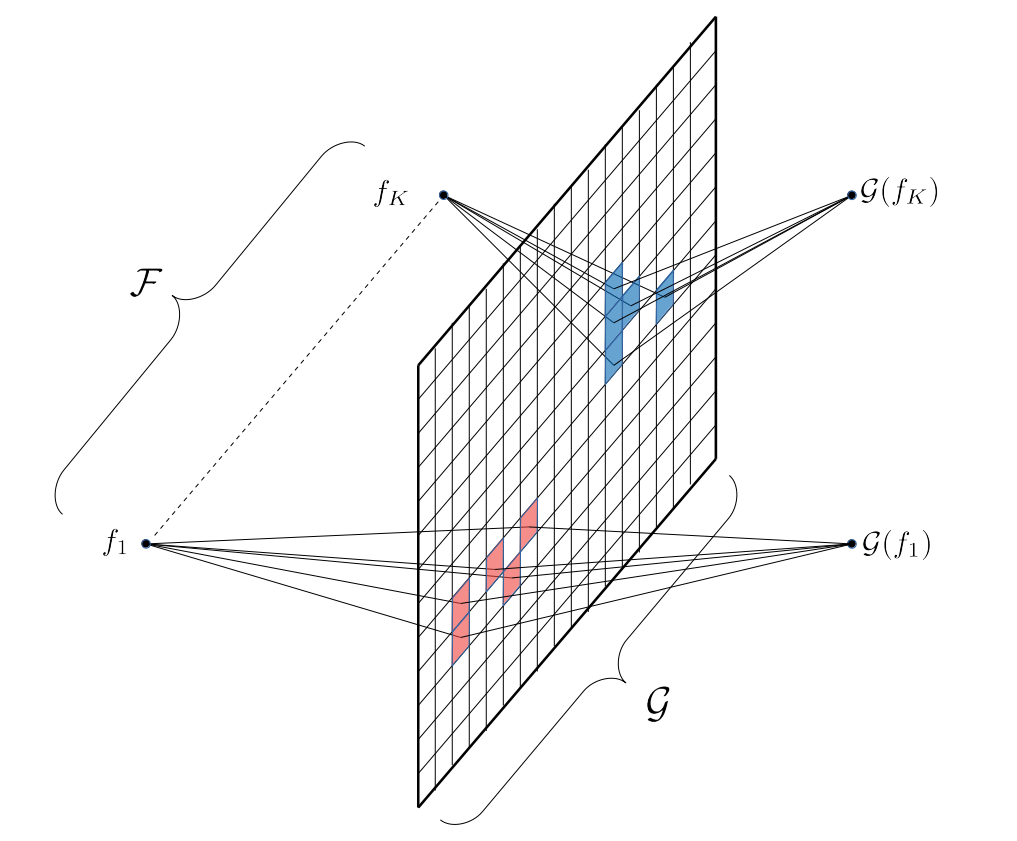
\includegraphics[scale=0.25]{figures/notations.png}
\end{figure}


\begin{itemize}
\item $\mathcal{G}$ the measure grid is a set of bit, $\mathcal{G} = \lbrace b_1, \ldots b_n \rbrace$.
\item $n$ the size of the measure grid, $\vert \mathcal{G} \vert = n$. 
\item $S(\mathcal{G})$  the set of all possible permutation of $\mathcal{G}$, $\vert S(\mathcal{G})\vert = 2^{n}$.
\item $S(\mathcal{G}, l)$  the set of all permutation of $\mathcal{G}$ of size $l$.
\item $\mathcal{F}$ the set of latent factor, $\mathcal{F} = \lbrace f_1, \ldots f_K \rbrace$.
\item $K$ the number of latent factor, $\vert \mathcal{F} \vert = K$.
\item $S(\mathcal{F})$  the set of all possible permutation of $\mathcal{F}$, $\vert S(\mathcal{F})\vert = 2^{K}$.
\item $S(\mathcal{F}, l)$  the set of all permutation of $\mathcal{F}$ of size $l$.
\item $\mathcal{G}(f)$  the set of bits activated by factor $f$, $\mathcal{G}(f) \in S(\mathcal{G})$ and $f \in \mathcal{F}$.  
\item $\mathcal{G}^{-1}(b)$  the set of factors that activate grid's bit $b$, $\mathcal{G}^{-1}(b) \in S(\mathcal{F})$ and $b \in \mathcal{G}$.
\end{itemize}

\section{Definitions And Properties}

\subsection{Statistical definitions}

In this section we provide formalism for the statistical description of factor's activity, there signature on the measure grid as well as the activation estimator.

\subsubsection*{Activation of factors}

Each factor takes value in $\{ 0, 1\}$ at each instant of time. A factor with value 1 at some instant is active otherwise it has value 0. At this stage of the paper we assume no particular statistical modelisation of factor. Nevertheless if we consider the set of all possible combination of active and unactive factors ($F(2)^{K}$), we assume that there is a well defined distribution $d'$ such that 

\begin{align*}
d' &: F(2)^{K} \rightarrow [0,1]\\
d'_x &= \mathbb{P}\left(f_1 = x_1, \ldots, f_K = x_K \right)
\end{align*}

Factors have statistical signatures on the measure grid. That is, there activation lead to the activation of bits of the measure grid. Again, at this stage only the minimum requirement are specified for its statistical modelisation. That is for any $I \in S(\mathcal{G})$

\begin{align*}
\mathbb{P}(\mathcal{G}(f) = I) &\in [0, 1]\\
\sum_{I \in S(\mathcal{G})} \mathbb{P}(\mathcal{G}(f) = I) &=1
\end{align*}

The modelisation of latent factor's activation and link to measure grid induce a distribution over combinations of activation of measure grid's bits. We refer to this distribution as $d$

\begin{align*}
d &: F(2)^{n} \rightarrow [0,1]\\
d_x &= \mathbb{P}\left(b_1 = x_1, \ldots, b_n = x_n \right)
\end{align*}

Furthermore, for $I \in S(\mathcal{F})$, the modelisation of latent factor to bit' s links verifies also 

\begin{align*}
\mathbb{P}(\mathcal{G}^{-1}(b) = I) &\in [0, 1]\\
\sum_{I \in S(\mathcal{F})} \mathbb{P}(\mathcal{G}^{-1}(b) = I) &=1
\end{align*}


\subsubsection*{Characteristic polynome}

The activity of a factors and grid's bit may be modelized using a set of multivariate polynomials whose fiber and image domain is respectively $F(2)^{n}$ and $F(2)$. $F(2)$ denotes the fields of two elements, $0$ and $1$, equipped with the logical XOR and logical AND as the addition and multiplication, respectively. The set of polynome associated with a set $I \in S(\mathcal{F})$ or $I' \in S(\mathcal{G})$ is denoted $\lbrace \mathcal{P}_{I, l} \rbrace_{l \in \mathbb{N}}$ and represents respectively a segmentation of states of factors and measure grid's bits in $I$ or $I'$. That is, in the measure grid's space space

\begin{align*}
\mathcal{P}_{I', l}&: F(2)^{n} \rightarrow F(2)\\
\mathcal{P}_{I', l} &= \begin{cases} \sum_{\pi \in S(I', l)} x_{\pi_1} \cdot x_{\pi_2} \cdot \ldots \cdot x_{\pi_l}, & \text{if }\ l \in \lbrace 1, \ldots, \vert I \vert \rbrace \\ 0, & \text{otherwise} \end{cases}
\end{align*}

Where $S(I", l)$ is the set of all permutation of size $l$ of element of $I'$ and $x_b \in F(2)$ is the state of a bit $b \in \mathcal{G}$. Furthermore we define the characteristic polynomial of the set of bits $I'$ at level $l_0 \in \{0, \ldots, \vert I' \vert \}$ as 

\begin{align*}
\mathcal{P}^{l_0}_{I'} &: F(2)^{n} \rightarrow F(2)\\
\mathcal{P}^{l_0}_{I'} &= \sum_{l = l_0}^{\vert I' \vert} \mathcal{P}_{I', l}
\end{align*}

The same polynomial can be expressed to modelize states of set of factors. So far, the addition is set to be the logical XOR in the definition of fields $F(2)$. However, in the rest of this report, we will use symbol $+$ and $\sum$ as representation of a logical OR in $F(2)$. This notation enables us to save a lot of time in writing complex polynomials. Denoting $\oplus$ the logical XOR and $\bar{x}$ the opposite of $x$, one have

\begin{equation*}
(x \cdot \bar{y}) \oplus (\bar{x} \cdot y) \oplus (x \cdot y) = x + y 
\end{equation*}  

\subsubsection*{Operators on polynome}

In order to qualify a set of factors and grid's bits, we define some basic operator. First, let  $I_{\mathcal{G}}$ some subset of $S(\mathcal{G})$. Then we denote by $F_2(I_{\mathcal{G}}, \mathcal{G})$ the operators that transform $I_{\mathcal{G}}$ into a set of $\vert I_{\mathcal{G}} \vert$ vector in $F(2)^{\vert \mathcal{G} \vert}$. 

\begin{equation*}
F_2(I_{\mathcal{G}}, \mathcal{G})  : S(\mathcal{G}) \rightarrow  F(2)^{\vert \mathcal{G} \vert \times \vert I_{\mathcal{G}} \vert} 
\end{equation*}

For each of the vector $X \in F_2(I_{\mathcal{G}}, \mathcal{G})$ that has been generated by corresponding set $I \in I_{\mathcal{G}}$, an entry takes value $1$ if the associated element belongs to $I$, 0 otherwise. This oprerator is convenient to evaluate the characteristic polynome of a set of grid's bit. As an example, let $I \in S(\mathcal{G})$ and $l_0 \in \{ 1, \ldots \vert I \vert \}$, then 

\begin{align*}
\sum_{x \in F_2(\lbrace I' \rbrace, \mathcal{G})} \mathcal{P}_I^{l_0} \left[ x \right]  &= \begin{cases} 1, & \text{if }\ \vert I'\cap I \vert \geq l_0 \\ 0, & \text{otherwise} \end{cases}
\end{align*}

With $I'$ any subset of $\mathcal{G}$. Let the ditribution over states of grid's bits be denoted $d = \lbrace d_x \rbrace_{x \in F_2(S(\mathcal{G}), \mathcal{G})}$ with $d_x = \mathbb{P}(X = x)$, Then the norm of a characteristic Polynome $\mathcal{P}_I^{l_0}$ with respect to distribution $d$ is defined as

\begin{align*}
\Vert . \Vert_{d} &: \mathcal{P}_{F_2(S(\mathcal{G}), \mathcal{G})} \rightarrow \left[ 0, 1\right] \\
\Vert \mathcal{P}_I^{l_0} \Vert_{d} &= \sum_{x \in F_2(S(\mathcal{G}), \mathcal{G})} \mathcal{P}_I^{l_0}\left[ x \right] \times d_x
\end{align*}


Where $ \forall x \in F_2(S(\mathcal{G}), \mathcal{G})$, $\mathcal{P}_{F_2(S(\mathcal{G}), \mathcal{G})}$ the space of all polynomials with domain $F_2(S(\mathcal{G}), \mathcal{G})$ and $\times$ is the simple multiplication in $\mathbb{R}$. Finally, keeping previous notations, let $\lbrace \mathcal{P}_{I_{i}}^{l_i} \rbrace_{i=1, ..., k}$ a set of characteristic polynome for some $k \in \mathbb{N}$, we define the product operator as 

\begin{align*}
\langle ., \ldots, . \rangle_{d} &: \mathcal{P}_{F_2(S(\mathcal{G}), \mathcal{G})}^{k} \rightarrow \left[ 0, 1\right] \\
\langle \mathcal{P}^{l_1}_{I_1}, \ldots,  \mathcal{P}^{l_k}_{I_k} \rangle_{d} &= \sum_{x \in F_2(S(\mathcal{G}), \mathcal{G})} \left( \mathcal{P}^{l_1}_{I_1} \left[ x \right] \cdot \ldots \cdot \mathcal{P}^{l_k}_{I_k} \left[ x \right] \right) \times d_x
\end{align*}

Where $\cdot$ denotes the usual multiplication in $F(2)$ and $\times$ is the simple multiplication in $\mathbb{R}$. Every operator specified above in the measure grid space can be defined in the factor space, taking distribution of factor's activation $d'$ and input domain $\mathcal{F}$ instead of distribution $d$ and input space $\mathcal{G}$.


\subsection{Firing Graph}
In this section we provide a description of the main datastructure used in our solution, the firing graph, as well as basic tools to help its analysis.
  
\subsubsection*{Graph specification}
The algorithm presented in this report use a particular datastructure that we refer as firing graph and that we denote $G(V, D_w)$. 

\begin{itemize}
\item $V$ is the set of vertice $V = \lbrace v_1, \ldots, v_{\vert V \vert} \rbrace$
\item $D_w$ is the weighted direct link matrix, $D_w \in \mathbb{N}^{\vert V \vert \times \vert V \vert}$ and $\left[ D_w \right]_{i, j} = w$ indicate an edge of weight $w$ from vertex $v_i$ to vertex $v_j$ if $w > 0$  
\end{itemize}

$G$ is a directed weighted graph whose vertice are organized in layer. A vertex of some layer $i \in \mathbb{N}$ must have at least one incoming edge from a vertex of layer $i-1$. It may also have outcoming edges toward vertice of layer $j \in \mathbb{N}, j > i$ and incoming edges from vertice of layer $k \in \mathbb{N}, k < i$. Vertice of layer $0$ has no incoming edges, they corresponds to bits of the measure grid $\mathcal{G}$. Each vertex stores the tuple $(I, l_0)$

\begin{itemize}
\item $I$ the set of vertice at the tail of incoming edge of the vertex
\item $l_0$ the firing rate's lower bound of the vertex, usually referred as level, $l_0 \in \lbrace 1, \ldots, \vert I \vert \rbrace$ 
\end{itemize}

 \begin{figure}[H]
 \centering
   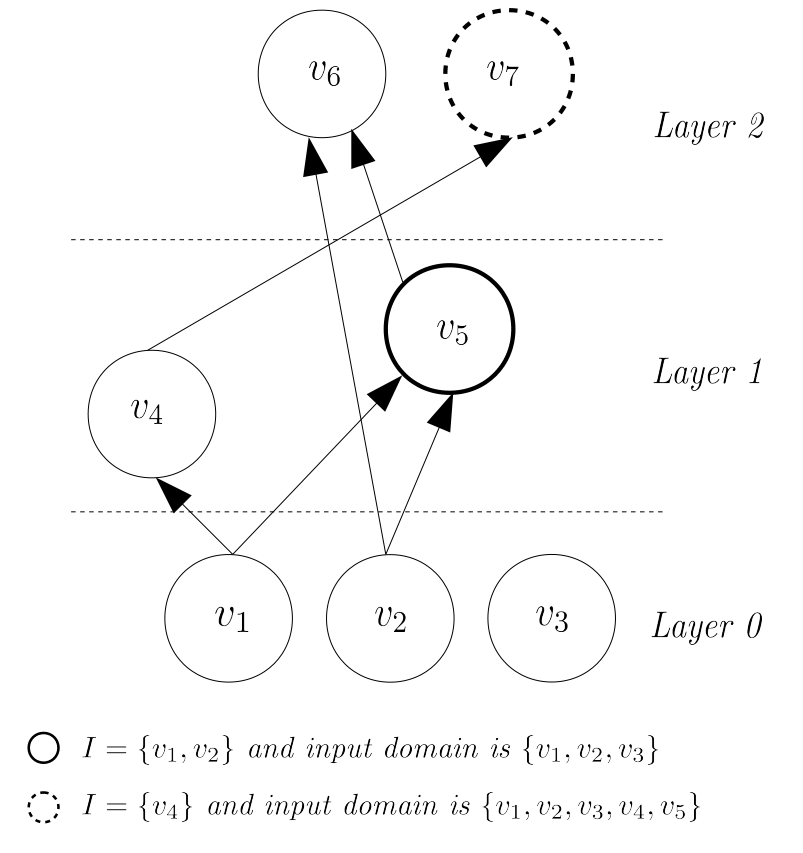
\includegraphics[scale=0.25]{figures/firing_graph.png}
\end{figure}

In the figure we introduce the input domain of a vertex $v$ of the firing graph. It corresponds to the set of vertice that are candidate for an egde toward $v$. Vertice of the firing graph can also be characterized by there state that can take value 0 or 1 and there propagation through the graph at a rate $\tau$ that needs to be set. If at an instant $t_0$ we set the state of each vertex of layer $0 \leq i < k$ for some $k > 0$, then at instant $t_1 = t_0 + \tau$ vertice of layer $k$ will have there state updated according to their incoming links. The propagation of states through the graph may be modelized by a multivariate boolean polynomial.

\subsubsection*{Graph Polynomials}

As we have previously defined the characteristic polynome of a set of grid's bit and factors, we associate to a vertex $v(I, l_0)$ of the firing graph $v$ the set of polynome $\lbrace \mathcal{P}_{I, l} \rbrace_{l \in \{l_0, \ldots, \vert I \vert \ \}}$ that represent a segmentation of the state of a vertex at instant $t$ given the state of vertex in its input domain at instant $t-\tau$ . If we denote by $n$, $I$ and $l_0$ respectively the size of the input domain of $v$, the set of vertex that has a link toward $v$ and the level of the vertex, then 

\begin{align*}
\mathcal{P}_{v, l}&: F(2)^{n} \rightarrow F(2)\\
\mathcal{P}_{v, l} &= \begin{cases} \sum_{\pi \in S(I, l)} x_{\pi_1} \cdot x_{\pi_2} \cdot \ldots \cdot x_{\pi_l}, & \text{if }\ l \in \lbrace l_0, \ldots, \vert I \vert \rbrace \\ 0, & \text{otherwise} \end{cases}
\end{align*}

Where $S(I, l)$ is the set of all permutation of size $l$ of element of $I$ and for any vertex $v \in V$, $x_{v} \in F(2)$, is the state of $v$. Furthermore we define the characteristic polynomial of a vertex $v$ as 

\begin{align*}
\mathcal{P}_v &: F(2)^{n} \rightarrow F(2)\\
\mathcal{P}_v &= \sum_{l = l_0}^{\vert I \vert} \mathcal{P}_{v, l}
\end{align*}

Again all operators on polynome defined previously is applicable, let $v$ be some vertex of the firing graph and $d_x$ a ditribution over the combination activation of $v$'s input domain, denoted $d = \lbrace d_x \rbrace_{x \in F_2(S(\mathcal{G}), \mathcal{G})}$ with $d_x = \mathbb{P}(X = x)$. Then the norm of $v$ with respect to distribution $d$ is defined as

\begin{equation*}
\Vert \mathcal{P}_v \Vert_{d} = \sum_{x \in F_2(S(\mathcal{G}), \mathcal{G})} \mathcal{P}_v\left[ x \right] \times d_x
\end{equation*}

Similarly, let $v_1, \ldots, v_k$ be any vertice of the firing graph with the same input domain and $d_x$ a ditribution over states of this input domain. Then the product with respect to distribution $d$ is defined as

\begin{equation*}
\langle \mathcal{P}_{v_1}, \ldots,  \mathcal{P}_{v_k} \rangle_{d} = \sum_{x \in F_2(S(\mathcal{G}), \mathcal{G})} \left( \mathcal{P}_{v_1} \left[ x \right] \cdot \ldots \cdot \mathcal{P}_{v_k} \left[ x \right] \right) \times d_x
\end{equation*}

\subsubsection*{Connection to grid's bit}

The firing graph is a convenient data structure to evaluate polynome of group of measure grid's bits. Let $G$ be a firing graph with its layer 0 composed of the set of bits $\mathcal{G}$, then for any vertext of layer 1 $v(I, \vert I \vert)$ the characteristic polynome $v$ is equal to the characteristic polynome of the set of bits $I \in \mathcal{G}$ with level $\vert I \vert$ decayed with a delay $\tau$

\begin{equation*}
\mathcal{P}_{v} = \mathcal{P}_{I, \vert I \vert}
\end{equation*}

Furthermore if we set the level of $v$ to 1 its characteristic polynome become the logical $or$-sum of the characteristic polynome of each bits of $I$, again delayed by $\tau$

\begin{equation*}
\mathcal{P}_{v} = \sum_{b \in I} \mathcal{P}_{\{ b \}, 1}
\end{equation*}

Finally one can design more complexed arrangement of vertice that enables to modelize multiple set of measure grid's bits. Let $G$ be a firing graph with its layer 0 composed of the set of bits $\mathcal{G}$, let $u(I, \vert I \vert)$ and $v(I', 1)$, such that $I \cap I' = \emptyset$, be vertice of layer 1 and $w(\{ u, v \}, 2)$ a vertex of layer 2. Then one can easily see that that characteristic polynome of $w$ verifies

\begin{equation*}
\mathcal{P}_{w} = \sum_{b \in I'} \mathcal{P}_{I \cup \{ b \}, \vert I \vert + 1}
\end{equation*}


Decayed with delay $2 \times \tau$.


\subsection{Evaluation of measure grid's bits}

A perfect indicator of the activation of a given factor $f$ can be used as target activation behaviour to evaluate the possibility of any set of bits to be part of the signature of the factor on the measure grid. 

\subsubsection*{Factor's signature}

The activation of factors can be modeled by a polynome in the factor space defined as 

\begin{align*}
\mathcal{P}_{f} &: F(2)^K \rightarrow F(2)\\
 \mathcal{P}_{f} &=  \mathcal{P}_{\{f\}, 1}
\end{align*}

Further we could also describe the activity of a factor $f$ by a polynome in the measure grid's space

\begin{align*}
\mathcal{P}_{\mathcal{G}(f)} &: F(2)^n \rightarrow F(2)\\
 \mathcal{P}_{\mathcal{G}(f)} &=  \mathcal{P}_{\mathcal{G}(f), \vert \mathcal{G}(f) \vert}
\end{align*}

The characterististic polynomes of a factor $f \in \mathcal{F}$ verifies $\forall$ $I \subset \mathcal{F}$ and $I' = \bigcup_{f' \in I} \mathcal{G}(f')$ let $x, x' \in F(2)^{K} \times F(2)^{n}$ such that $x \in F_2(\{I\}, \mathcal{F})$ and $x' \in F_2(\{I'\}, \mathcal{G})$
\begin{center}
$\mathcal{P}_f[x] = 1 \Rightarrow \mathcal{P}_{\mathcal{G}(f)}[x'] = 1$
\end{center}

Furthermore if $!\exists J \in \mathcal{F} \setminus \{ f \}$ such that $\mathcal{G}(f) \subset \bigcup_{f' \in J} \mathcal{G}(f')$

\begin{center}
$\mathcal{P}_f[x] = 1 \Leftrightarrow \mathcal{P}_{\mathcal{G}(f)}[x'] = 1$
\end{center}

\subsubsection*{basic metrics}

Let $I \in S(\mathcal{G})$, $l \in \{ 1, \ldots, \vert I \vert \}$, $f \in \mathcal{F}$ and $e$ be respectively some measure grid's bit, some level, some latent factor and the event "factor f is active". Then we define a first metrics, refered as recall coefficient, defined as

\begin{equation*}
\mu_{I, l, f} = \langle \mathcal{P}^{l}_{I}, \mathcal{P}_{\mathcal{G}(f)} \rangle_{d \vert e} + \langle \mathcal{P}^{l}_{I}, \mathcal{P}_{\mathcal{G}(f)}^{\bot} \rangle_{d \vert e}
\end{equation*}

Where $d \vert e$ is the  distribution over measure grid's bits activation given event $e$ and $\mathcal{P}_{\mathcal{G}(f)}^{\bot}$ is the complement of $\mathcal{P}_{\mathcal{G}(f)}$ in $F(2)$. Furthermore we define the precision coefficient as

\begin{equation*}
\nu_{I, l, f} = \langle \mathcal{P}^{l}_{I}, \mathcal{P}_{\mathcal{G}(f)} \rangle_{d \vert \bar{e}} + \langle \mathcal{P}^{l}_{I}, \mathcal{P}_{\mathcal{G}(f)}^{\bot} \rangle_{d \vert \bar{e}}
\end{equation*}

Where $d \vert \bar{e}$ is the  distribution over measure grid's bits activation given not event $e$. Finally we define the purity coefficient as 

\begin{equation*}
\omega_{I, l, f} = \frac{\nu_{I, l, f}}{\mu_{I, l, f}}
\end{equation*}


The lower $\omega_{I, l, f}$ the more pure is the set $I$ with respect to $f$. Furthermore one can easily see that for any set $I \in S(\mathcal{G})$ we have 

\begin{equation*}
\omega_{I,l, f} \geq \omega_{\mathcal{G}(f), \vert \mathcal{G}(f) \vert, f}
\end{equation*}

Finally the recall, precision and purity coefficient can be defined for any vertex $v$ of a firing graph where vertex of layer 0 are composed by measure grid's bit and are denoted respectively $\mu_{v, f}$, $\nu_{v, f}$ and $\omega_{v, f}$.

\subsubsection*{advanced metrics}

 
Let $I \in S(\mathcal{G})$, $l \in \{ 1, \ldots, \vert I \vert \}$, $f \in \mathcal{F}$ and $e$ be respectively some measure grid's bit, some integer, some latent factor and the event "factor f is active". Then we define the precision of the set $I$ with respect to factor $f$ at level $l_0$ as

\begin{equation*}
\phi_{I, l, f} = \frac{\Vert \mathcal{P}^{l}_I \Vert_{d, e}}{\Vert \mathcal{P}^{l}_I \Vert_{d}}
\end{equation*}

We also define the recall of the set $I$ with respect to factor $f$ at level $l_0$ as

\begin{equation*}
\psi_{I, l, f} = \frac{\Vert \mathcal{P}^{l}_I \Vert_{d, e}}{\Vert \mathcal{P}_{\mathcal{G}(f)} \Vert_{d, e}}
\end{equation*}

Where $d, e$ is a well defined distribution over combination of activation of measure grid's bits that intetersect with event $e$. Finally the precision and the metrics can be defined for any vertex $v$ of a firing graph where vertex of layer 0 are composed by measure grid's bit and are denoted respectively $\phi_{v, f}$ and $\psi_{v, f}$.

\subsubsection*{Stochastic process induced by vertex}

Given that the layer 0 of the firing graph is compose of measure grid's bits, the propagation of activation through the firing graph induces multiple stochastic processus in each of its vertex. Given a vertex $v$ at layer $k \geq 0$, its  characteristic polynome $\mathcal{P}_{v}$, a factor $f$ and its characteristic polynome in the measure grid space $\mathcal{P}_f$ the activity of the node is described by
 
\begin{itemize}
\item The firing process, $n_{v}\left[ t \right]$, $t \in \mathbb{N}$\\

$n_{v}\left[ t \right] = n_{v}\left[ t - \tau \right] + n_{v, t}$ with $\lbrace n_{v, t} \rbrace_{t \in \mathbb{N}}$ a set of i.i.d random variable that takes value 1 when vertex $v$ activate. That is, $\forall$ $t  < k \times \tau $, $n_{v, t} = 0$ and $\forall$ $t  \geq k \times \tau $ \\ 
\begin{center}
$n_{v, t} = \begin{cases} 1, & \text{with probability } q_n = \Vert \mathcal{P}_{v} \Vert_d  \\ 0, & \text{with probability } 1 - q_n \end{cases}$
\end{center}

Where $d$ is the distribution over combination of activation of vertice of layer 0. 

\item The reward process with respect to factor $f$, $r_{v, f} \left[ t \right]$, $t \in \mathbb{N}$\\

$r_{v, f} \left[ t \right] = r_{v, f} \left[ t - \tau \right] + r_{v, t, f}$, with $\lbrace r_{v, t, f} \rbrace_{t \in \mathbb{N}}$ a set of i.i.d random variable that takes value 1 if vertex $v$ activate at instant $t$ and the event "factor $f$ activate" was true at time $t - k \times \tau$. That is,  $\forall$ $t  < k \times \tau $, $r_{v, t, f} = 0$ and $\forall$ $t  \geq k \times \tau $\\ 
\begin{center}
$r_{v, t, f} = \begin{cases} 1, & \text{with probability } q_r = \Vert \mathcal{P}_{v} \Vert_{d, e} \\  0, & \text{with probability } 1 - q_r  \end{cases}$
\end{center}

where $d, e$ is the distribution over the combination of activation of vertex of layer 0 that intersect with the event e: "factor $f$ is active".

\item The penalty process with respect to factor $f$, $p_{v, f}\left[ t \right]$, $t \in \mathbb{N}$\\

$p_{v, f}\left[ t \right] = p_{v, f}\left[ t - \tau\right] + p_{v, t, f}$, with $\lbrace p_{v,t, f} \rbrace_{t \in \mathbb{N}}$ a set of i.i.d random variable that takes value 1 if vertex $v$ activate at instant $t$ and the event "factor $f$ activate" was false at time $t - k \times \tau$. That is, $\forall$ $t  < k \times \tau $, $p_{v, t, f} = 0$ and $\forall$ $t  \geq k \times \tau $\\ 

\begin{center}
$p_{v, t, f} = \begin{cases} 1, & \text{with probability } q_p = q_n - q_r \\ 0, & \text{with probability } 1 - q_p \end{cases}$
\end{center}


\item The score process with respect to factor $f$, $s_{v, f}\left[N, T, \rho \right]$, $N, T, \rho \in \mathbb{N}^3$ \\

$s_{v,f}\left[N, T, \rho \right] = N + \sum_{t=1}^{T} s_{v, \rho, t, f}$, with $\lbrace s_{v, \rho, t, f} \rbrace_{t \in \mathbb{N}}$ a set of i.i.d random variable. $s_{v, \rho, t, f}$ takes value 1 if the event "factor $f$ activate" was true at time $t - k \times \tau$ and value $-\rho$ if the event was false, given that $v$ activate at $t$. That is, $\forall$ $t  < k \times \tau $, $p_{v, t, f} = 0$ and $\forall$ $t  \geq k \times \tau $\\ 

\begin{center}
$s_{v, \rho, t, f} = \begin{cases} 1, & \text{with probability } q_s = \frac{q_r}{q_r + q_p}  \\ -\rho, & \text{with probability } 1 - q_s \end{cases}$
\end{center}
\end{itemize}

The stochastic processus of each vertex is a convenient way to estimate the evaluation metrics of sets of measure grids bit's whose behaviour is caught be a vertex of the firing graph.

\subsection{Properties}

This paragraph intend to deliver useful properties for the analysis of the algorithm. The proof of every properties can be found in the appendice at the end of this paper.

\subsubsection*{Polynomial decomposition}

\underline{Partition}\\

Let $v_1(I, l_0)$, $v_2(J, 0)$ and $v_3(K, 0)$, be three vertice of the same firing graph, with the same input domain $\mathcal{G}$ such that $I = J \cup K$ and $J \cap K = \emptyset$, then, $\forall x \in F_2(S(\mathcal{G}), \mathcal{G})$

\begin{equation}
\mathcal{P}_I^{l_0}\left[ x \right] = \sum_{l=l_0}^{\vert I \vert} \sum_{j=0}^{\vert J \vert} \mathcal{P}_{J, j}\left[ x \right]  \cdot \mathcal{P}_{K, l - j}\left[ x \right] 
\end{equation} 

In paticular for $v \in I$

\begin{equation}
\mathcal{P}_{I, l}\left[ x \right] = \mathcal{P}_{I\setminus \{ v\}, l}\left[ x \right] \cdot \mathcal{P}_{\{ v\}, 0}\left[ x \right] + \mathcal{P}_{I\setminus \{ v\}, l-1}\left[ x \right] \cdot \mathcal{P}_{\{ v\}, 1}\left[ x \right]
\end{equation} 

\underline{Decomposition}\\

Let $G$ be a firing graph composed of a set of $\mathcal{G}$ of vertice of layer 0. $u(I, l_u)$, $v(I', l_v)$ such that $I \cap I' = \emptyset$ as vertice of layer 1 and $w(\{ u, v \}, 2)$ as vertex of layer 2. Let $K \in S(I', l_v)$ then 


\begin{equation}
\label{prop:2layer-1}
\mathcal{P}_{K, \vert K \vert} \cdot \mathcal{P}_{\{u, v\}, 2} = \sum_{l=l_u}^{\vert I \vert}  \sum_{J \in S(I, l)} \mathcal{P}_{J \cup K, l + \vert K \vert }
\end{equation}

In particular if $l_u = \vert I \vert$ and $l_u = 1$ , then for any vertex of layer 0 $v\in I'$

\begin{equation}
\label{prop:2layer-2}
 \mathcal{P}_{b, 1} \cdot \mathcal{P}_{\{u, v\}, 2} = \mathcal{P}_{I \cup \{b\}, \vert I \vert + 1}
\end{equation}


\subsubsection*{Metrics}

Throughout this section, we consider a firing graph $G$ where the layer 0 is composed by measure grid's bits. $v$ denote some vertex of $G$ and $f \mathcal{F}$ denote some factor. Finally we use  $d$ and $d'$ to respectively denote the distribution over combination of activation of measure grid's bits and factors and $e$ to denote the event "factor $f$ is active". \\

\underline{Precision of vertex}\\

Let $v$ be a vertex connected to a set $I$ subset of vertex of its input domain and let $f \in \mathcal{F}$ be some factor. Then the precision of $v$ with respect to $f$ is

\begin{equation}
\label{prop:precision1}
\phi_{v, f} = \frac{\Vert \mathcal{P}_{f} \Vert_{d'}}{\Vert \mathcal{P}_{f} \Vert_{d'} + (1 - \Vert \mathcal{P}_{f} \Vert_{d'}) \times \omega_{v, f}}
\end{equation}

Furthermore we have

\begin{equation}
\phi_{v, f} \leq \frac{\Vert \mathcal{P}_{f} \Vert_{d'}}{\Vert \mathcal{P}_{f} \Vert_{d'} + (1 - \Vert \mathcal{P}_{f} \Vert_{d'}) \times \omega_{\mathcal{G}(f),\vert \mathcal{G}(f) \vert, f}} 
\end{equation}

\underline{Recall of vertex}\\

Let $v$ be a vertex connected to a set $I$ of vertex of its input domain and let $f \in \mathcal{F}$ be some factor. Then the recall of $v$ with respect to $f$ is

\begin{equation}
\psi_{v, f} = \mu_{v, f}
\end{equation}

Furthermore, 

\begin{equation}
0 \leq \phi_{v, f} \leq 1
\end{equation}

Where right equality is reached whenever $v$ is connected to a set of measure grid's bit $I \in \mathcal{G}$, with level $l_0 = \vert I \vert$ such that $I \subset \mathcal{G}(f)$. 


\subsubsection*{stochastic processus}

Again, throughout this section, we consider a firing graph $G$ where the layer 0 is composed by measure grid's bits. $v$ denote some vertex of $G$ and $f \mathcal{F}$ denote some factor. Finally we use  $d$ and $d'$ to respectively denote the distribution over combination of activation of measure grid's bits and factors and $e$ to denote the event "factor $f$ is active". \\

\underline{vertex's reward process}\\

If denotes penalty process of $v$ with respect to $f$ as defined in section 1.2.2, then

\begin{equation}
\mathbb{E} \left[ r_{v, f}[t]  \right] = t \times q_r = t \times (\mu_{v, f} \times \Vert \mathcal{P}_{f} \Vert_{d'})
\end{equation}

\underline{vertex's penalty process}\\

if $p_{v, f}[t]$ denotes penalty process of $v$ with respect to $f$ as defined in section 1.2.2, then

\begin{equation}
\mathbb{E} \left[ p_{v, f}[t]  \right] =  t \times q_p = t \times ( \nu_{I, f} \times (1 -\Vert \mathcal{P}_{f} \Vert_{d'}))
\end{equation}

\underline{vertex's score process}\\

If $s_{v, f}[N, T, \rho]$ denotes the score process of $v$ with respect to $f$ as defined in section 1.2.2 with some $N, T, \rho \in \mathbb{N}^3$, then

\begin{equation}
\label{prop:score_mean}
\mathbb{E} \left[ s_{v, f}[N, T, \rho]  \right] = N + T \times (q_s\times (\rho + 1) - \rho) = N + T \times (\phi_{v, f} \times (\rho + 1) - \rho)
\end{equation}

Furthermore,

\begin{equation}
\label{prop:score_var}
\Var \left[ s_{v,\rho, t, f}  \right] = ???
\end{equation}

\section{Identification of Latent Factor}
In this section, we presents the a couple of operations that can be used for the identification of a latent factor:

\begin{itemize}
\item Sampling: Sampling the measure grid and build a firing graph
\item Draining: Draining vertex of the firing graph keeping only low purity coefficient's vertex
\end{itemize}

At this stage both processus will be described and the efficiency of the draining algorithm quantified.

\subsection{Sampling}


The sampling of the measure grid is a specific procedure followed in order to select some bits of the grid. This procedure is usually designed to be the most efficient in the fullfilment of specific quantitative objective. First we assume that given a target factor $f$ we have access to a determinist exact indicator of $f$'s activation. Then given target $f$, the objective of our sampling is to maximize the probability that we sample a bit $b$ whose purity coefficient with respect to $f$ is higher or equal to some positive constant $\omega^{*}$. That is, if we denote by $s$ the random variable of the outcome of a single sampling, then the objective is to maximize

\begin{center}
$\mathbb{P}( \omega_{\{s\}, 1, f} \geq \omega^{*})$
\end{center}  

Again if we have a set of $I \subset \mathcal{G}$ bits, a target factor $f$, then the objective of sampling is to maximize the probability of sampling a bit $b$ for which the purity of set $I \cup \{b \}$ is higher or equal to a given positive constant $\omega^{*}$. That is, if we denote by $s$ the random variable of the outcome of a single sampling, then the objective is to maximize

\begin{center}
$\mathbb{P}( \omega_{I \cup \{ s\}, \vert I \vert, f} \geq \nu)$
\end{center} 

Since we assume a perfect indicator of activation of latent factor, we propose a very intuitive sampling method. Given parameters $n_s\in \mathbb{N}^{*}$ and $p_s \in [0, 1]$ the sampling procedure is 

ALGORITHM PSEUDO CODE LIKE 

The second mean of the sampling procedure is to build a firing graph from which the evaluation of the purity coefficient of samples can be estimated through the observation of their score process. We will focus on two particular case

\subsubsection*{The case where no bits has been pre-selected}

 \begin{figure}[H]
 \centering
   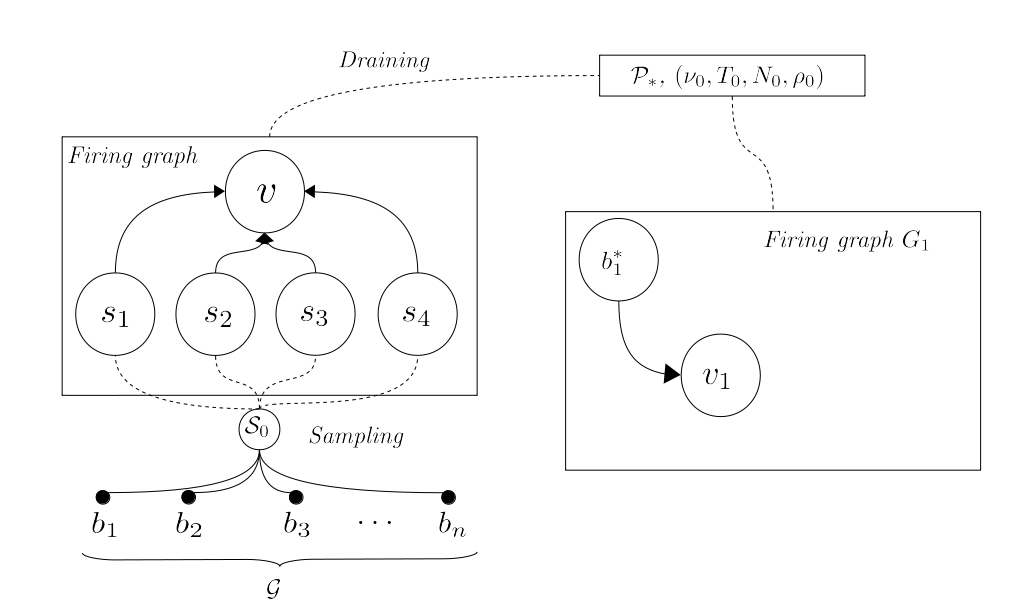
\includegraphics[scale=0.43]{figures/iteration_0.png}
\end{figure}

In this case blabla

\subsubsection*{The case where some bits has been preselected}

 \begin{figure}[H]
 \centering
   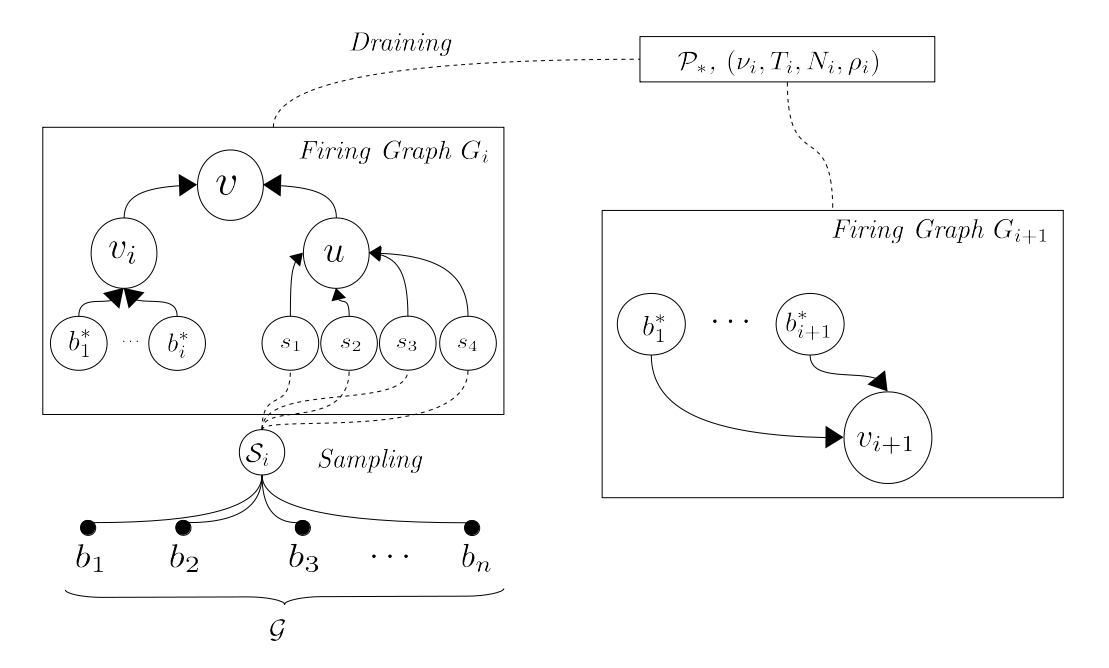
\includegraphics[scale=0.40]{figures/iteration_i.png}
\end{figure}

In this case blabla

\subsection{Draining}


The algorithm takes as input a sequence of 4-tuple $(\omega^{*}, N, T, \rho_i)$ and a target factor $f$.


\subsection{Analysis of the algorithm}

\begin{theorem}
\label{th_stopping}
Given a sampling strategy $\mathcal{S}$, a set of pre-selected bits $I =\{b_{1}^{*}, \ldots, b_{i}^{*}\}$ and a target factor $f$. There exists a 4-tuple $(\omega, N, T, \rho)$ such that the probability that the firing graph $G$ has a capacity 0 at the end of the of draining is upper bounded. More specifically, given that $S$ is the set of sampled bits.

\begin{equation*}
\mathbb{P} \left( G \textit{ has capacity 0} \right) \leq \sum_{j = 0}^{\vert S \vert} p^j \times \mathbb{P}_{\mathcal{S}} \left( \vert \lbrace s \in S \setminus \omega_{I \cup \{s\}, \vert I \vert + 1, f } < \omega \rbrace \vert = j \right) 
\end{equation*}

Where $p = \mathbb{P} \left( s_{v, f}(N, T, \rho < 0) \vert \omega_{I \cup \{ s \}, i + 1, f} < \omega_i \right)$, with $\{b_1^{*}, \ldots, b_{i}^{*}, s \}$ vertices of the layer 0 and $v(I \cup \{ s \}, i+1)$ at the layer 1 of a firing graph of depth 2, Furthermore

\begin{equation*}
\mathbb{P} \left( s_{v, f}(N, T, \rho < 0) \vert \omega_{I \cup \{ s \}, i + 1, f} < \omega \right) \leq C \times \max \left( \exp\left(- T \times \left(\frac{\delta^{+}\delta_{i,f} c}{\sigma}\right)^2 \right), \exp\left(- T \times \delta^{+}\delta_{i,f}c \right) \right)
\end{equation*}

With $\delta_{i, f}$, $\delta^+$ $C$ and $c$ are postitive constants that depends on $\omega$ and $i$ and $\Var[s_{v, \rho, t}] = \sigma^2$. 

\end{theorem}

\begin{leftbar}
\textbf{Proof.} As a reminder, in the core of this proof we refer to $d$ and $d'$ respectively to the distribution over bit's grid activation and factor's activation. Given the arrangement of vertex of graph $G$ built with sampling and using (\ref{prop:2layer-2}), the characteritic polynomial of any of the  vertex $s$ composing layer 0 of $G$ that correspond to bits sampled write as

\begin{equation*}
\mathcal{P}_{s}= \mathcal{P}_{\{b^{*}_1, \ldots, b^{*}_i, s \}, i+1}
\end{equation*}

As a consequence, the score process of each vertex sampled $s$ in $G$ is equal to the score process of a vertex $v(\{b^{*}_1, \ldots b^{*}_i, s \}, i+1)$ at layer 1 of a graph of two layers where $ \{b^{*}_1, \ldots b^{*}_i, s \}$ composes its layer 0. Then, the first inequality is trivial, since it consists in a naive development. Indeed 

\begin{align*}
\mathbb{P} \left( L_i = \emptyset \vert L_{i-1} \neq \emptyset  \right) &= \sum_{j=0}^{\vert S \vert} p^j \times q^{\vert S \vert -j} \times\mathbb{P}_{\mathcal{S}_i} \left( \vert \lbrace s \in S \setminus \omega_{I \cup \{s\}, i + 1, f } < \omega_i \rbrace \vert = j \right) \\
&\leq \sum_{i=0}^{\vert S \vert} p^i \times \mathbb{P}_{\mathcal{S}_i} \left( \vert \lbrace s \in S \setminus \omega_{I \cup \{s\}, i + 1, f } < \omega_i \rbrace \vert = i \right)
\end{align*}  

Where 
\begin{itemize}
\item $I =\{b_{1}^{*}, \ldots, b_{i}^{*}\}$
\item $p = \mathbb{P} \left( s_{v, f}(N_i, T_i, \rho_i) < 0 \vert \omega_{I\cup\{s \}, i + 1, f} < \omega_i \right)$
\item $q = \mathbb{P} \left( s_{v, f}(N_i, T_i, \rho_i) < 0 \vert \omega_{I\cup\{s \}, i + 1, f} \geq \omega_i \right)$
\end{itemize}

Then, we choose the value of the postive real $\omega_i$ such that there exists a bit $b^{+}$ that verifies

\begin{align*}
b^{+} = &\argmin_{b \in \mathcal{G}} \vert \omega_i - \omega_{I \cup \{ b \}, i +1, f} \vert \\
&\textit{ such that } \omega_i - \omega_{I \cup \{ b \}, i +1, f} > 0 
\end{align*}

And we define the vertex $v^{+}(I \cup \{b^{+}\}, i+1)$ and $\delta^{+} = \vert \omega_i - \omega_{v^{+}, f} \vert$. If vertex $v$ is such that $\omega_{v,f}  < \omega_i$ then using (\ref{prop:precision1}) one get 

\begin{equation*}
\underbrace{\frac{\Vert \mathcal{P}_{f} \Vert_{d'}}{\Vert \mathcal{P}_{f} \Vert_{d'} + (\omega_i - \delta) \times (1 - \Vert \mathcal{P}_{f} \Vert_{d'})}}_{\phi_{v, f}} \geq \underbrace{\frac{\Vert \mathcal{P}_{f} \Vert_{d'}}{\Vert \mathcal{P}_{f} \Vert_{d'} + (\nu_i - \delta^{+}) \times (1 - \Vert \mathcal{P}_{f} \Vert_{d'})}}_{\phi_{v^{+}, f}} \geq \underbrace{\frac{\Vert \mathcal{P}_{f} \Vert_{d'}}{\Vert \mathcal{P}_{f} \Vert_{d'} + \omega_i  \times (1 - \Vert \mathcal{P}_{f} \Vert_{d'})}}_{\phi_i}
\end{equation*}

For some real $\delta > \delta^{+} > 0$. Then, We choose the 3-tuple $(N_i, T_i, \rho_i)$ as follow:

\begin{align*}
\rho_i &= \textit{min } \rho \in \mathbb{N} \textit{ such that } \phi_i \times (\rho+1) - \rho < 0\\
N_i &= -t \times (\phi_i \times (\rho_i+1) - \rho_i )\\
T_i &= t
\end{align*}

for any $t \in \mathbb{N}^{*}$. Now considering $v$ with $\omega_{v,f}  < \omega_i$ one can write

\begin{align*}
\mathbb{P} \left( s_{v,f}[N_i, T_i, \rho_i] < 0 \right) &= \mathbb{P} \left( N_i + \sum_{t=1}^{T_i} s_{v, \rho_i, T_i, f} < 0 \right) \\
&= \mathbb{P}\left( \sum_{t=1}^{T_i} s_{v, \rho_i, t, f} - T_i \times \mathbb{E}\left[s_{v, \rho_i, 1, f}\right] < -N_i -  T_i \times \mathbb{E}\left[s_{v, \rho_i, 1, f}\right]\right)
\end{align*}

Yet using equation (\ref{prop:score_mean}) one have

\begin{align*}
\mathbb{E}\left[s_{v, \rho_i, 1, f}\right] &= \phi_{v, f} \times (\rho_i + 1) - \rho_i\\
&= \frac{\Vert \mathcal{P}_{f} \Vert_{d'}}{\Vert \mathcal{P}_{f} \Vert_{d'} + (\omega_i - \delta)  \times (1 - \Vert \mathcal{P}_{f} \Vert_{d'})} \times (\rho_i + 1) - \rho_i
\end{align*}

Furthermore using $T_i = t$ and $N_i = t \times \left(\phi_i (\rho_i + 1) - \rho_i \right)$ and the definition of $\phi_i$ one have

\begin{equation*}
-N_i -  T_i \times \mathbb{E}\left[s_{v, \rho_i, 1, f}\right] = -t \times \delta \times \underbrace{(\rho_i +1) \times \phi_i \times \phi_{v, f} \times \frac{1 - \Vert \mathcal{P}_{f} \Vert_{d'}}{\Vert \mathcal{P}_{f} \Vert_{d'}}}_{\delta_{i, v, f}}
\end{equation*}

Thus

\begin{align*}
\mathbb{P} \left( s_{v,f}[N_i, T_i, \rho_i] < 0 \right) &= \mathbb{P}\left( \sum_{t=0}^{T_i - 1} s_{v, \rho_i, t, f} - \mathbb{E}\left[s_{v, \rho_i, t, f}\right] < -t \times \delta \times \delta_{i, v, f} \right)\\
&\leq \mathbb{P}\left(\vert \sum_{t=0}^{T_i - 1} s_{v, \rho_i,t, f} - \mathbb{E}\left[s_{v, \rho_i, t, f}\right] \vert > t \times \delta \times \delta_{i, v, f} \right)\\
&\leq \mathbb{P}\left(\vert \sum_{t=0}^{T_i - 1} s_{v, \rho_i, t, f} - \mathbb{E}\left[s_{v, \rho_i, t, f}\right] \vert > t \times \delta^{+} \times \delta_{i, f} \right)
\end{align*}

With $\delta_{i, f} = (\rho_i +1) \times \phi_i^{2} \times \frac{1 - \Vert \mathcal{P}_{f} \Vert_{d'}}{\Vert \mathcal{P}_{f} \Vert_{d'}}$. \\

At this point we have to notice that $\lbrace s_{v, \rho_i, t, f} \rbrace_{t=1, \ldots, T_i - 1}$ is a sequence of i.i.d random variables with mean $\mu$ and variance $\sigma^2$ that verifies $\vert s_{v, \rho_i, t, f} \vert \leq \rho_i$. Thus one can apply the Chernoff inequality as formulated in \cite{TAO-1}. In particular, taking $\lambda = \sigma^{-1} \delta^{+} \delta_{i,f}$ we obtain

\begin{align*}
\mathbb{P}\left(\vert \sum_{t=0}^{T_i - 1} s_{v, \rho_i, tn f} - \mathbb{E}\left[s_{v, \rho_i, t, f}\right] \vert > t \delta^{+} \delta_{i,f} \right) &= \mathbb{P}\left(\vert \sum_{t=0}^{T_i - 1} s_{v, \rho_i, t} - \mathbb{E}\left[s_{v, \rho_i, t}\right] \vert > \lambda\sigma \sqrt{t} \right)\\
&\leq C \times \max \left( \exp\left(- t \times \left(\frac{\delta^{+}\delta_{i,f} c}{\sigma}\right)^2 \right), \exp\left(- t \times \delta^{+}\delta_{i,f}c \right) \right)
\end{align*}


With $C, c$ some positive constant and $\Var[s_{v, \rho_i, t, f}] = \sigma^2$. Q.E.D.

\end{leftbar}

\begin{theorem}
\label{th_precision}
Given a sequence of sampling strategy $\lbrace \mathcal{S}_i \rbrace_{i=0, \ldots, n-1}$, a target factor $f$. There exists a sequence of 4-tuple $\lbrace (\omega_i, N_i, T_i, \rho_i) \rbrace_{i=0, \ldots, n-1}$ such that, at iteration $i$,  Given a set of sampled bits $S$,

\begin{equation}
\mathbb{P} \left( \phi_{v_{i+1}} < \phi_i \right)\leq \mathbb{E}_{\mathcal{S}_i}\left[  \vert \lbrace b \in S \setminus \omega_{I \cup \{b\}, i + 1, f } < \omega_i \rbrace \vert\right] \times p
\end{equation}

Where $I =\{b_{1}^{*}, \ldots, b_{i}^{*}\}$, $p = \mathbb{P} \left( s_{v, f}(N_i, T_i, \rho_i) > 0 \vert \omega_{I \cup \{ s \}, i + 1, f} > \omega_i \right)$, $\{b_1^{*}, \ldots, b_{i}^{*}, s \}$ are placed at the layer 0 and $v(I \cup \{ s \}, i+1)$ at the layer 1 of a firing graph, Furthermore

\begin{equation*}
p \leq C \times \max \left( \exp\left(- t \times \left(\frac{\delta^{-}\delta_{i,f} c}{\sigma}\right)^2 \right), \exp\left(- t \times \delta^{-}\delta_{i,f}c \right) \right)
\end{equation*}

With $C, c$ two postitive constant, $\delta^-$ a constant that depends on $\omega_i$ and $\Var[s_{v, \rho_i, t, f}] = \sigma^2$. 
\end{theorem}

\begin{leftbar}
\textbf{Proof.} First $v_{i+1}$ is the vertex with input set $I \cup \{ b^{*}_{i+1}\}$ and level $i +1$, where $I = \{b^{*}_1, \ldots, b^{*}_i \}$ and $b^{*}_{i+1}$ is the bit that has been selected at the end of current iteration's drainer routine. Again, using a similar argument (\ref{prop:2layer-2}) than in the previous proof, one can show that the score process of each vertex $s$ at layer 0 of $G_i$ sampled at iteration i, is equal to the score process of a vertex $v(\{b^{*}_1, \ldots b^{*}_i, s \})$ at layer 1 of a graph of 2 layers where $ \{b^{*}_1, \ldots b^{*}_i, s \}$ composes it's layer 0. Let also $S$ be the set of sampled measure grid's bit at iteration i that compose the layer 0 of a the firing graph. Then one can write

\begin{equation*}
\mathbb{P} \left( \phi_{v_{i+1}, f} >  \phi_i \right) = \sum_{k = 1}^{\vert S \vert} \mathbb{P}_{\mathcal{S}_i} \left( \vert \lbrace s \in S \setminus \omega_{I \cup \{s\}, i + 1, f } > \omega_i \rbrace \vert = k \right) \times \sum_{l=1}^{k} \sum_{l'=0}^{\vert S \vert -k} p_{l, k} \times q_{l', \vert S \vert - k} \times \frac{l}{l + l'}
\end{equation*}

where

\begin{align*}
p_{l, k} &= \begin{pmatrix} l \\ k  \end{pmatrix} \times p \times (1 -p )^{k-l} \\
q_{l', k} &= \begin{pmatrix} l' \\ \vert S \vert - k  \end{pmatrix} \times q^{l} \times (1 -q )^{\vert S \vert -k-l}
\end{align*}

With 

\begin{align*}
p &= \mathbb{P} \left( s_{v, f}(N_i, T_i, \rho_i) > 0 \vert \omega_{I \cup \{ b \}, i + 1, f} > \omega_i \right)\\
q &= \mathbb{P} \left( s_{v, f}(N_i, T_i, \rho_i) > 0 \vert \omega_{I \cup \{ b \}, i + 1, f} < \omega_i \right)
\end{align*}

Where $b \in S$ and $v(I \cup \{s\}, i+1)$ a vertex of layer 1 of a firing graph with layer 0 composed of $I \cup \{s\}$. Thus

\begin{align*}
\mathbb{P} \left( \phi_{v_{i+1}, f} >  \phi_i \right) &\leq \sum_{k = 0}^{\vert S \vert} k \times \mathbb{P}_{\mathcal{S}_i} \left( \vert \lbrace s \in S \setminus \omega_{I \cup \{s\}, i + 1, f } < \omega_i \rbrace \vert = k \right) \times p  \\
&= \mathbb{E}_{\mathcal{S}_i}\left[  \vert \lbrace s \in S \setminus \omega_{I \cup \{s\}, i + 1, f } < \omega_i \rbrace \vert\right] \times p
\end{align*}

Then, we choose the value of the postive real $\omega_i$ such that there exists a bit $b^{-}$ that verifies

\begin{align*}
b^{-} = &\argmin_{b \in \mathcal{G}} \vert \omega_i - \omega_{I \cup \{ b \}, f} \vert \\
&\textit{ such that } \omega_i - \omega_{I \cup \{ b \}, f} < 0 
\end{align*}

And we define the vertex $v^{-}(I \cup \{b^{-}\}, i+1)$ and $\delta^{-} = \vert \omega_i - \omega_{v^{-}, f} \vert$. If $v$ is such that $\omega_{v, f}  < \omega_i$ then using (\ref{prop:precision1}) we have 

\begin{equation*}
\underbrace{\frac{\Vert \mathcal{P}_{f} \Vert_{d'}}{\Vert \mathcal{P}_{f} \Vert_{d'} + (\omega_i + \delta) \times (1-\Vert \mathcal{P}_{f} \Vert_{d'})}}_{\phi_{v, f}} \leq \underbrace{\frac{\Vert \mathcal{P}_{f} \Vert_{d'}}{\Vert \mathcal{P}_{f} \Vert_{d'} + (\omega_i + \delta^{-}) \times (1 - \Vert \mathcal{P}_{f} \Vert_{d'})}}_{\phi_{v^{-}, f}} \leq \underbrace{\frac{\Vert \mathcal{P}_{f} \Vert_{d'}}{\Vert \mathcal{P}_{f} \Vert_{d'} + \omega_i \times (1 - \Vert \mathcal{P}_{f} \Vert_{d'})}}_{\phi_i}
\end{equation*}

for some $\delta \geq \delta^{-} > 0$. Then defining the 3-tuple $(N_i, T_i, \rho_i)$ as

\begin{align*}
\rho_i &= \textit{min } \rho \in \mathbb{N} \textit{ such that } \phi_i \times (\rho+1) - \rho < 0\\
N_i &= -t \times (\phi_i \times (\rho_i+1) - \rho_i ) \times \mu_{v, f} \\
T_i &= t 
\end{align*}

for any $t \in \mathbb{N}^{*}$. Now considering $v$ with $\omega_{v,f}  > \omega_i$, reproducing the same development as it was done in the proof of previous Theorem, one can derive a convenient form to easily apply the Chenoff inequality.

\begin{equation*}
\mathbb{P} \left( s_{v, f}(N_i, T_i, \rho_i) > 0 \vert \omega_{v, f} > \omega_i \right) \leq \mathbb{P}\left(\vert \sum_{t=0}^{T_i - 1} s_{v, \rho_i, t, f} - \mathbb{E}\left[s_{v, \rho_i, t, f}\right] \vert > t \times \delta^{-} \delta_{i,f} \right)
\end{equation*}

With $\delta_{i, f} = (\rho_i +1) \times \phi_i^{2} \times \frac{1 - \Vert \mathcal{P}_{f} \Vert_{d'}}{\Vert \mathcal{P}_{f} \Vert_{d'}}$. Then using the Chernoff inequality as written in \cite{TAO-1} using $\lambda = \sigma^{-1} \delta^{+} \delta_{i,f}$ we obtain


\begin{align*}
\mathbb{P}\left(\vert \sum_{t=0}^{T_i - 1} s_{v, \rho_i, t, f} - \mathbb{E}\left[s_{v, \rho_i, t, f}\right] \vert > T_i \times \mu_{v, f}\delta^{-} \rho_i \right) \leq C \times \max \left( \exp\left(- t \times \left(\frac{\delta^{-}\delta_{i,f} c}{\sigma}\right)^2 \right), \exp\left(- t \times \delta^{-}\delta_{i,f}c \right) \right)
\end{align*}

With $C, c$ some positive constant and $\Var[s_{v, \rho_i, t, f}] = \sigma^2$. Q.E.D

\end{leftbar}

The combination of Theorems shows that, given a sampling strategy, there exists a decreasing sequence of positive value $\lbrace \omega_i\rbrace_{i=1,\ldots, n-1}$ with a sequence of 3-tuple $\lbrace (N_i, T_i, \rho_i)\rbrace_{i=1,\ldots, n-1}$ such that when $t\rightarrow +\infty$ the probability that the algorithm output an optimal identificator of target factor $f$ tends to 1. it also highlights the trade-off between efficiency and complexity of the algorithm embodied in the choice of $\omega_i$ and $t$, on which depends $N_i$ and $T_i$ for $i=1, \ldots, n-1$.

\subsection{Limit of the generic case}

This generic case and its analysis deliver a strong framework that ease the derivation of more specific result that may be obtained under specific distribution of latent factors activation and link to measure grid. Nevertheless it leaves two fundamental points for the practical success of an algorithm clueless 

\begin{itemize}
\item What is a good choice of sequence of sampling strategy $\lbrace \mathcal{S}_0, \ldots, \mathcal{S}_{n-1} \rbrace$  
\item Is there any good procedure or heuristic to choose the sequence of decreasing positive real value $(\omega_0,\ldots, \omega_{n-1})$ ?
\end{itemize}

In the rest of this paper, we present two different specific cases of factor's and measure grid's modelisation that defines both sampling strategy and choice of $(\omega_0,\ldots, \omega_{n-1})$. 

\section{Case of signal plus noise}

This particular case is designed to be very easy to analyze. We first define the statistical signature of factor and bit's activation. Then we args a choice for the sequence 4-tuple $(\omega_i, T_i, N_i, \rho_i)_{i=1, \ldots, n-1}$. Finally we present simulations and provide discussion of the result obtained with this special case.

\subsection{Statistical modelisation}

In this particular case we assume that the target factor $f$ is linked to some $\vert \mathcal{G}(f)\vert = k$ measure grid's bits and activate with probability $p_f$. We also assume that bits of the measure grid are identically and independently subject to a noisy activation with probability $p_N$. We may see those noisy activation as the result of activation of $n$ noisy latent factor which are linked to exactly 1 bit of the measure grid, that is $K=n + 1$. Under this modelisation, the probability for a bit $b\in \mathcal{G}$ to activate is defined as 

\begin{equation*}
\mathbb{P} \left( \textit{"b active"} \right) = \begin{cases} p_{f} + p_N \times (1-p_{f}), & \text{if }\ b \in \mathcal{G}(f^{*}) \\ p_N, & \text{Otherwise} \end{cases}
\end{equation*}

As a consequence, for any $I \in S(\mathcal{G})$ such that $\vert I \cap \mathcal{G}(f) \vert = i$ and $j = \vert I \vert -i$ if we set $x\in F(2)^{n}$ such that $x \in F_2 (\{I\} , \mathcal{G})$, the distribution over measure grid bit's activation is defined as

\begin{equation*}
d_{x} =  \begin{cases} p_N^{i+j} \times (1-p_N)^{n - i - j} \times (1- p_{*}) + p_N^{j} \times (1-p_N)^{n - k - j} \times p_{*}, & \text{if }\ i=k \\ p_N^{i+j} \times (1-p_N)^{n - i - j} \times (1- p_{*}), & \text{Otherwise} \end{cases}
\end{equation*}

The rest of the section will always refer to this distribution as $d$.

\subsection{Evaluation of bits}

Let $G$ be a firing graph with a layer 0 composed of measure grid's bits. Then, the precision of a vertex $v(I,  \vert I \vert)$ of layer 1 of $G$ with respect to $f$ depends only on $\vert I \vert$ and $\vert I \cap \mathcal{G}(f) \vert$. Indeed, if $\vert I \cap \mathcal{G}(f) \vert = i$ then

\begin{equation*}
\phi_{v,f} = \frac{p_{f}}{p_{f} + (1 - p_{f})\times p_N^{i}}
\end{equation*}

With identification of terms using (\ref{prop:precision1}) we have $\omega_{v, f} = p_N^{i}$ and using previously defined distribution, one find that $\mu_{v, f} = p_N^{\vert I \vert - i}$, $\nu_{v, f} = p_N^{\vert I \vert}$. Besides, given a set of bits $I$, such that  $I \subset \mathcal{G}(f)$, for any bit $b \in \mathcal{G} \setminus I$ if $b \in \mathcal{G}(f)$ the precision of vertex $v(I \cup \{ b \}, \vert I \vert +1)$ with respect to $f$ is 

\begin{equation*}
\phi_{v} = \frac{p_{f}}{p_{f} + (1 - p_{f})\times p_N^{\vert I \vert + 1}}
\end{equation*}

if  $b \notin \mathcal{G}(f)$

\begin{equation*}
\phi_{v} = \frac{p_{f}}{p_{f} + (1 - p_{f})\times p_N^{\vert I \vert}}
\end{equation*}


\subsection{Sampling Strategy}

We define the initial sampling strategy $\mathcal{S}_0$ as the sampling of every activated bit of the measure grid at some instant when $f$ is active. The sampling strategy $\lbrace \mathcal{S}_i \rbrace_{i=1, \ldots, n-1}$ is then defined as 

\begin{equation*}
 \mathcal{S}_i : \begin{cases} \textit{Select all bits of } L_{i-1} \setminus \{ b^{*}_1, \ldots, b^{*}_{i'}\}, & \text{if }\ L_{i-1} \setminus\{ b^{*}_1, \ldots, b^{*}_{i'}\} \neq \emptyset \\ \mathcal{S}_0, & \text{ otherwise} \end{cases}
\end{equation*}

Where $\{ b^{*}_1,\ldots, b^{*}_{i'}\}$ is the set of previously selected bits, $i' \leq i$. Using the previously defined statistical distribution of bits activation, if we denote $S$ the set of sampled bits using $\mathcal{S}_0$, then the distribution of the cardinal of $S$ is 

\begin{align*}
\mathbb{P}\left(\vert S \vert = s\right) = \begin{cases} \begin{pmatrix} n - k \\ s - k  \end{pmatrix} \times p_N^{s - k } \times (1 - p_N)^{n-k-s}, & \text{if }\ s \geq k \\ 0, & \text{otherwise} \end{cases}
\end{align*}

Thus its expected size is $\mathbb{E}\left[ \vert S \vert \right] = k + (n - k) \times p_N $.

\subsection{Identification of factors}

In this particular case we follow the procedure described in the generic case except for the stopping criteria. Here we allow set $L_i$, to be empty if $i < \tau$, $\tau \in \mathbb{N}$ is to be set. Then we follow a specific procedure to choose the sequence $\lbrace \omega_i \rbrace_{i=0, n-1}$. First, at iteration 0, one can see that bit's purity coefficients can take only two values with respect to $f$

\begin{align*}
\omega_{\{b\}, 1, f} = \begin{cases} p_n , & \text{if }\ b \in \mathcal{G}(f) \\ 1, & \text{otherwise} \end{cases}
\end{align*}

Thus we choose 

\begin{equation*}
\omega_0 = \frac{(1 + p_N)}{2}
\end{equation*}

So to maximize the purity margin defined as
 
\begin{align*}
\delta_0 &=  \frac{(\omega_0 - \omega_{\{ b \}, 1, f}) + (\omega_{\{ b' \}, 1, f} - \omega_0)}{2} = \frac{(1-p_N)}{2}
\end{align*}

Where $b \in \mathcal{G}(f)$ and $b \notin \mathcal{G}(f)$. At iteration $i$, if we assume that the set $I$ is composed of all previously selected bits and verifies $\forall b \in I$, $b \in \mathcal{G}(f)$. Then remaining bit's purity coefficients with respect to $f$ can take again two values

\begin{align*}
\omega_{I \cup \{b\}, i+1, f} = \begin{cases} p_n^{i+1} , & \text{if }\ b \in \mathcal{G}(f) \\ pn^{i}, & \text{otherwise} \end{cases}
\end{align*}

Thus we choose

\begin{equation*}
\omega_i = \frac{(1 + p_N) \times p_N^{i}}{2}
\end{equation*}

gives the maximum purity margin
 
\begin{align*}
\delta_i &=  \frac{(\omega_i - \omega_{I \cup \{ b \}, i+1, f}) + (\omega_{I \cup \{ b' \}, i+1, f} - \omega_i)}{2} = \frac{(1-p_N) \times p_N^{i}}{2}
\end{align*}

Where $b \in \mathcal{G}(f)$ and $b \notin \mathcal{G}(f)$. Finally we define the sequence of 3-tuple $\lbrace (N_i, T_i, \rho_i) \rbrace_{i=1, \ldots}$ as 

\begin{align*}
\rho_i &= \textit{min } \rho \in \mathbb{N} \textit{ such that } \phi_i \times (\rho+1) - \rho < 0\\
N_{i} &= -t \times (\phi_i \times (\rho_i+1) - \rho_i )  \\
T_i &= t 
\end{align*}

Where $t \in \mathbb{N}$ and $\phi_i = \frac{p_{f}}{p_{f} + \omega_i \times (1 - p_f)}$.

\subsection{Simulation}

\section{Case of sparse measure grid}

This particular case is a bit more complex since we assume randomness of linked between latent factor and measure grid's bits. Again, for this particular case, we first define the statistical signature of factor and bit's activation. Then we args a choice for the sequence 4-tuple $(\omega_i, T_i, N_i, \rho_i)_{i=1, \ldots, n-1}$. Finally we present simulations and provide discussion of the result obtained with this sparse case.

\subsection{Statistical modelisation}


\subsubsection*{Latent factor activation}

We assume that activation of each of the $K$ latent factors is identical and independant. We denote by $p_f$ the probability of a latent factor's activation. As a consequence, for any $I \in S(\mathcal{F})$, if we define $x$ such that $x \in F_2 (\{I\}, \mathcal{F})$ then we can define the distribution of factor's activation as 

\begin{equation*}
d'_x = \times p_f^{\vert I \vert} \times (1-p_f)^{K-\vert I \vert} 
\end{equation*}


\subsubsection*{Measure grid activation}

We assume two major properties of activation of measure grid's bits.

\begin{itemize}
\item For each factor $f \in \mathcal{F}$, each bit $b \in \mathcal{G}$ has equal probability $p_g$ to belong to $\mathcal{G}(f)$.
\item For each factor $f \in \mathcal{F}$, for each couple $b_1, b_2 \in \mathcal{G}^2$, events "$b_1 \in \mathcal{G}(f)$" and "$b_2 \in \mathcal{G}(f)$"  are independent.
\end{itemize}   

As a consequence the probability for a bit $b$ to activate, given that every factor of some set $\{f_1, \ldots, f_k\} \subset \mathcal{F}$ is active write

\begin{align*}
\mathbb{P}\left(\textit{b active } \vert f_1, \ldots, f_k \textit{ active}\right) &= \sum_{i=1}^{k} \begin{pmatrix} k \\ i \end{pmatrix} \times p^i_g \times (1 - p_g)^{k - i}\\
 &= 1 - (1 - p_g)^{ k}
\end{align*}

The above quantity depends only on the number of active latent factor. Thus, for any $I \in S(\mathcal{G})$, if we define $x$ such that $x \in F_2 (S(\mathcal{G}) , \mathcal{G})$ then we can define the distribution of bits's activation as 

\begin{equation*}
d_x = \sum_{k = 1}^{K} \left[ \begin{pmatrix} K \\ k \end{pmatrix} \times p_f^{k} \times (1-p_f)^{K-k}\right] \times \left[ p^i_{g \vert k} \times (1 - p_{g\vert k})^{n - i} \right]
\end{equation*}

With $i = \vert I \vert$ and $p_{g \vert k} = \mathbb{P}\left(\textit{b active } \vert f_1, \ldots, f_k \textit{ active}\right)$.

\subsection{Evaluation of bits}

Let $G$ be a firing graph whose layer 0 is composed of measure grid's bits, given a target factor $f$, the precision with respect to $f$ of a vertex $v(\{ b \}, 1)$ of the layer 1 of $G$ depends on $b \in \mathcal{G}(f)$ and $\vert \mathcal{G}^{-1}(b) \vert$. Indeed if $b \in \mathcal{G}(f)$ and $\vert \mathcal{G}^{-1}(b) \vert = l$, its precision with respect to $f$ writes

\begin{equation*}
\phi_{v, f} = \frac{p_f}{p_f + (1 - p_f)\times \omega_{v, f}}
\end{equation*}

where $\omega_l = 1 - (1-p_f)^{l-1}$. If $b' \notin \mathcal{G}(f)$ and $\vert \mathcal{G}^{-1}(b') \vert = l$ then $v'(\{ b' \}, 1)$ verifies $\mu_{v', f} = \nu_{v', f} = (1 - (1-p_f)^{l})$. Thus its precision with respect to $f$ writes

\begin{equation*}
\phi_{v', f} = p_f
\end{equation*}

Futhermore if we have a vertex $v(I, \vert I \vert)$ such that $\forall b \in I$, $b \in \mathcal{G}(f)$ and $\min_{b \in I} \vert \mathcal{G}^{-1}(b) \vert = l$, then the precision of $v$ with respect to $f$ verifies

\begin{equation*}
\phi_{v, f} \leq \frac{p_f}{p_f + \omega^{-}_l \times (1 - pf)}
\end{equation*}

With 

\begin{equation*}
\omega^{-}_l = \sum_{k=K-l-1}^{K} \begin{pmatrix} K \\ k \end{pmatrix} p_f^{k} \times (1-p_f)^{K - k}
\end{equation*}

The minimum possible purity coefficient one can obtained with bits that verifies $b \in \mathcal{G}(f)$ and $\vert \mathcal{G}^{-1}(b) \vert = l$. That is the case of a vertex $v(I, \vert I \vert)$ with $I$ composed of every possible $\begin{pmatrix} K \\ l \end{pmatrix}$ such bits.


\subsection{Sampling Strategy}

In this special case we take the same sampling strategy as in the special case: signal plus noise. That is 

\begin{equation*}
 \mathcal{S}_i : \begin{cases} \textit{Select all bits of } L_{i-1} \setminus \{ b^{*}_1, \ldots, b^{*}_i\}, & \text{if }\ L_{i-1} \setminus\{ b^{*}_1, \ldots, b^{*}_i\} \neq \emptyset \\ \mathcal{S}_0, & \text{ otherwise} \end{cases}
\end{equation*}

Where $\{ b^{*}_1,\ldots, b^{*}_i\}$ is the set of previously selected bits and $\mathcal{S}_0$ consists in sampling every activated bit of the measure grid at some instant when $f^{*}$ is active. The computation of the expected number of bits sampled using $\mathcal{S}_0$ can be derived using defined distribution introduced previously.

 
\subsection{Identification of factors}
Again in this case we follow the procedure described in the generic case with stopping criteria $L_i = \emptyset$ and  $i \geq \tau$, $\tau \in \mathbb{N}$ is to be set. In addition we do not use a uniform strategy to select the bit from $L_i$ at the end of the $i^{th}$ iteration. We propose two distinct procedures for the choice of $\lbrace \omega_i \rbrace_{i=0, n-1}$.

\subsubsection*{Initialisation procedure}

We set $\omega_0$ to be equal to $\omega_l$ for some $l$ set reasonably small. Then if $L_0 = \emptyset$ we increment $l$ and set $\omega_1$ to $\omega_{l+1}$. We repeat this procedure up to the point where $L_p \neq \emptyset$ for some $p \geq 0$. Refering to Theorem \ref{th_precision} Any bit $b \in L_p$ is likely to respect $\omega_{\{b \}, f} \leq \omega_{l+p}$. 
 
\subsubsection*{Main procedure}

Let $p$ be such that $L_p = \{ b_1, \ldots, b_k \}$ is the first non empty set obtained with the initialisation procedure. Then we choose the bit $b_p^{*}$ from $L_p$ that is the vertex of the firing graph $G_{p}$ that has the highest score process value with respect to target factor $f$. Then, denoting by $\omega_{p}^{*}$ its purity coefficient, we set $\omega_{p+1} = \omega_{p}^{*}$. Again, at the end of $q^{th}$ iteration of main procedure, if $L_{p+q} \neq \emptyset$ then we choose the bit $b_{p+q}^{*}$ from $L_{p+q}$ that is the vertex of the firing graph $G_{p+q}$ that has the highest score process value with respect to target factor $f$ and set $\omega_{p+q+1}$ to its purity coefficient.\\


Finally we choose the sequence of 3-tuple $\lbrace (N_i, T_i, \rho_i) \rbrace_{i=1, \ldots}$ as 

\begin{align*}
\rho_i &= \textit{min } \rho \in \mathbb{N} \textit{ such that } \phi_i \times (\rho+1) - \rho < 0\\
N_i &= -t \times (\phi_i \times (\rho_i+1) - \rho_i )\\
T_i &= t 
\end{align*}

For some $t \in \mathbb{N}$ and  $\phi_i = \frac{p_f}{p_f + \omega_i \times (1-p_f)}$. 

\subsection{Simulation}
Important note for practice $\nu$ can be estimated using $R=$ the reward process value divided by target behaviour firing process and $P$ the penalty process: $\nu = \frac{P}{R}$
\newpage
\bibliography{mybib}{}
\bibliographystyle{plain}

\end{document}

